\documentclass[a4paper,12pt]{article}
\usepackage[utf8]{inputenc}
\usepackage[english]{babel}
\usepackage{amssymb,amsmath,graphicx,listings}
\usepackage{uniinput}
\usepackage[left=2cm,right=2cm,top=2cm,bottom=2cm]{geometry}
\renewcommand{\familydefault}{\sfdefault}
\newcommand{\leadingzero}[1]{\ifnum #1<10 0\the#1\else\the#1\fi}
\newcommand{\mytoday}{\leadingzero{\day}.\leadingzero{\month}.\the\year}
\newcommand{\code}[1]{\textit{#1}}

\lstset{language=matlab, numbers=left,numberstyle=\footnotesize, basicstyle=\footnotesize}


\begin{document}
\title{Semester project TMA4215}
\author{10068 and 728387}
\date{\mytoday}
\maketitle
%\newpage


\section{Task}
We consider minimization problems of the type
\begin{align*}
\min_{{\bf x} \in \mathbb{R}^n} g({\bf x}),\,\, g({\bf x}):=-{\bf b}^T{\bf x} + \frac12{\bf x}^TH{\bf x}+\frac1{12}{\bf x}^TC({\bf x}){\bf x},
\end{align*}
here ${\bf b} \in \mathbb{R}^n$ and, $H$ is a $n \times n$ symmetric and positive definite matrix and $C(\bf{x})$ is a diagonal
matrix with diagonal entries $c_i x^2_i, i = 1, . . . , n$. 
Here $c_i > 0$ are the components of a vector ${\bf c} \in \mathbb{R}^n$ 
and $x_i$ are the components of $\bf{x}$. 

\section{Mathematical calculations}
At first some calculations are done.
\subsection{Positive definition of $H$}\label{definit}
Since we use only one $H$, the proof is not generally, but only for one special matrix.
Let $u=\begin{pmatrix}u_1\\u_2\end{pmatrix}\in \mathbb{R}^2\backslash \begin{pmatrix}0\\0\end{pmatrix}$, and $H= \begin{pmatrix} a&b\\b&c\end{pmatrix}$, with $a,c>0$.
\begin{align*}
{\bf u}^TH{\bf u} = au_1^2 + cu_2^2 + 2 b u_1u_2
\end{align*}
If we choose $b = \sqrt{a}\sqrt{c}$, we get
$$ = (\sqrt{a}u_1+\sqrt{c}u_1)^2 >0,$$
no matter what ${\bf u}$ is. 
$H$ is positive definite with this choice of $b$.

\subsection{Gradient}
The gradient can easily be calculated with sums.
\begin{align*}
{\bf\nabla} g 
&= {\bf \nabla}\left(-\sum_{i=1}^nb_ix_i +\frac12\sum_{i=1}^n\sum_{j=1}^n H_{ij}x_ix_j + \frac1{12}\sum_{i=1}^n c_i x_i^4\right)
\end{align*}
The two sums in the middle are divided into the diagonal element and the not diagonal elements.
All not diagonal elements are there twice, because $H$ is symmetric and therefore $H_{ij} = H_{ji}$ .
\begin{align*}
&= {\bf \nabla}\left(-\sum_{i=1}^nb_ix_i +\frac12\sum_{i=1}^n H_{ii}x_i^2 + \sum_{i=1}^n\sum_{j=1}^{i-1} H_{ij}x_ix_j + \frac1{12}\sum_{i=1}^n c_i x_i^4\right)
\\&= -{\bf b} + H{\bf x} + \frac13C{\bf x}
\end{align*}

\subsection{Hessian}
The Hessian of $g$ is easily calculable:
\begin{align*}
{\bf\nabla}^2 g =  H + C
\end{align*}

\subsection{Existence of minimum}
Let $u\in R^n$ be an arbitrary vector, except $\vec{0}$ then
$$u^T(\nabla^2g(x))u = u^T (H+C) u = u^T H u + u^TCu = u^THu + \sum_{i=1}^n c_iu_i^2x_i^2.$$
Since $H$ is positive definite, $u^THu>0$ and because $c_i>0$, $u^TCu>0$, so 
$$u^T(\nabla^2g(x))u>0$$ 
That means that the Hessian of $g$ is positive definite and therefore strictly convex and has at most one local minimum.

\subsection{Equivalence of steepest decent method and forward Euler method}


\subsection{Optimal $α$ in the steepest decent method}\label{calcalpha}
To find the optimal $α$,
$$
g\left({\bf x}^{(k+1)}\right) = g \left({\bf x}^{(k)} - α^{(k)} \nabla g({\bf x}^{(k+1)})\right)
$$
has to be minimal, so $\frac{∂}{∂α} g({\bf x}^{(k+1)})$  has to be zero.
This leads to the equation
\begin{align*}
f=&\left( {\bf b}{\bf \nabla} g - {\bf x}  \left(H+\frac{C}{3}\right)  {\bf \nabla} g\right)
 + \left( ({\bf \nabla} g) ( H + C) {\bf \nabla} g \right)α
\\+ &\left( - \sum_{i=1}^n c_i  x_i  ({\bf \nabla} g)_i^3 \right)α^2
+ \frac13\left( \sum_{i=1}^n c_i  ({\bf \nabla} g)_i^4\right)α^3 
\\ &= a_0 + a_1 α + a_2 α^2 + a_3α^3= 0
\end{align*}
Since the function is a cubic polynomial, the limit for 
$\lim_{α\rightarrow \pm\infty}f=\pm\infty$
and because the function is continuous, there has to be at least one real zero.

The function is always rising. So only one zero is possible.


\section{Main algorithms}
\subsection{Generation of the data}
The data is generated in the function \code{data}.

\begin{lstlisting}
function [ b, H, c ] = data
	b = [ 1; 0 ];
	c = [ 200; 400 ];
	H = [ 200, 20 ; 20, 2 ];
end
\end{lstlisting}
With the calculations in chapter \ref{definit} can be easily seen that $H$ is positive definite.

\subsection{Function, gradient and Hessian of $g$}

\begin{lstlisting}
function [ g ] = g ( X )
	[ b, H, c ] = data;
	dim = size(H,1);
	C = zeros ( dim, dim );
	for i = 1 : dim
		C(i,i) = c(i) * X(i) * X(i);
	end
	g = - b' * X + 0.5 * X' * H * X + 1/12 * X' * C * X;
end
\end{lstlisting}

\begin{lstlisting}
function [ nablaG ] = grad( X )
	[ b, H, c ] = data;
	dim = size ( H, 1 );
	for i = 1 : dim
	    C(i,i) = c(i) * X(i) * X(i);
	end
	nablaG = - b + H * X + 1/3 * C * X;
end
\end{lstlisting}

\begin{lstlisting}
function [ hessG ] = hessian( X )
	[ ~, H, c ] = data;
	dim = size ( H, 1 );
	C = zeros ( dim, dim );
	for i = 1 : dim
		C(i,i) = c(i) * X(i) * X(i);
	end
	hessG = H + C;
end
\end{lstlisting}

\subsection{Minimum searching algorithm}\label{core}
All methods work similar, only line 9 has to be exchanged.
The real implementation is more complicated and is shown in the next chapter.
\begin{lstlisting}
X = [ 4; -1 ];
maxiterations = 20;
tol = 1e-8;

norm_old = norm ( grad ( X) );
condition = 1;
while condition
	maxiterations = maxiterations - 1;
	X = X - alpha * grad ( X ); % steepest decent method with constant alpha
	% X = X - optimalAlpha ( X ) * grad ( X ); % with optimal alpha
	% X = X - linsolve ( hessian ( X ), grad ( X ) ); % newton method
	residual = norm ( grad ( X ) ) / norm_old;
	condition = (maxiterations > 0) && ( residual > tol);
end
\end{lstlisting}

\subsection{Computation of α}
For the calculation of α see chapter \ref{calcalpha}.
\begin{lstlisting}
function [ alpha_optimal ] = optimalAlpha( X )
[ b, H, c] = data;
dim = size ( H, 2 );
C = zeros ( dim, dim );
gradg = grad ( X );
a3 = 0;
a2 = 0;
for i = 1 : dim
	C(i,i) = c(i) * X(i)^2;
	a3 = a3 + c(i) / 3 * gradg(i)^4;
	a2 = a2 - c(i) * X(i) * gradg(i)^3;
end
a1 = gradg' * ( H + C ) * gradg;
a0 = b'*gradg - X' * H * gradg - 1/3 * X' * C * gradg;
alphas = roots( [ a3, a2, a1, a0 ] );
for i = 1 : 3
	if imag ( alphas ( i ) ) == 0
		alpha_optimal = alphas ( i );
	end
end
end
\end{lstlisting}
 
\section{Structure of the project}
The project can be started by executing \code{main()}. 
There the initial guess, the tolerance and the maximal number of iterations is defined. 
\code{main} first calls \code{plotmethod}, which contains a variant of the code in chapter \ref{core} and returns the relative residuals, and the points ${\bf x}^{k}$.
The change of $\bf x$ in each iteration is calculated in \code{delta} for various methods.
At the end of \code{main}, all plots are generated using the functions \code{drawfunction} and \code{drawcurve}.

\section{Results}
With the program presented above, several experiments can be done.
If not other stated, $(4,-1)^T$ is used as initial guess, $10^{-8}$ as tolerance and the number of iterations is limited to $20$.
A first look at the function with the defined values suggest the minimum is around $(0,0)^T$.
\begin{figure}\label{g}
	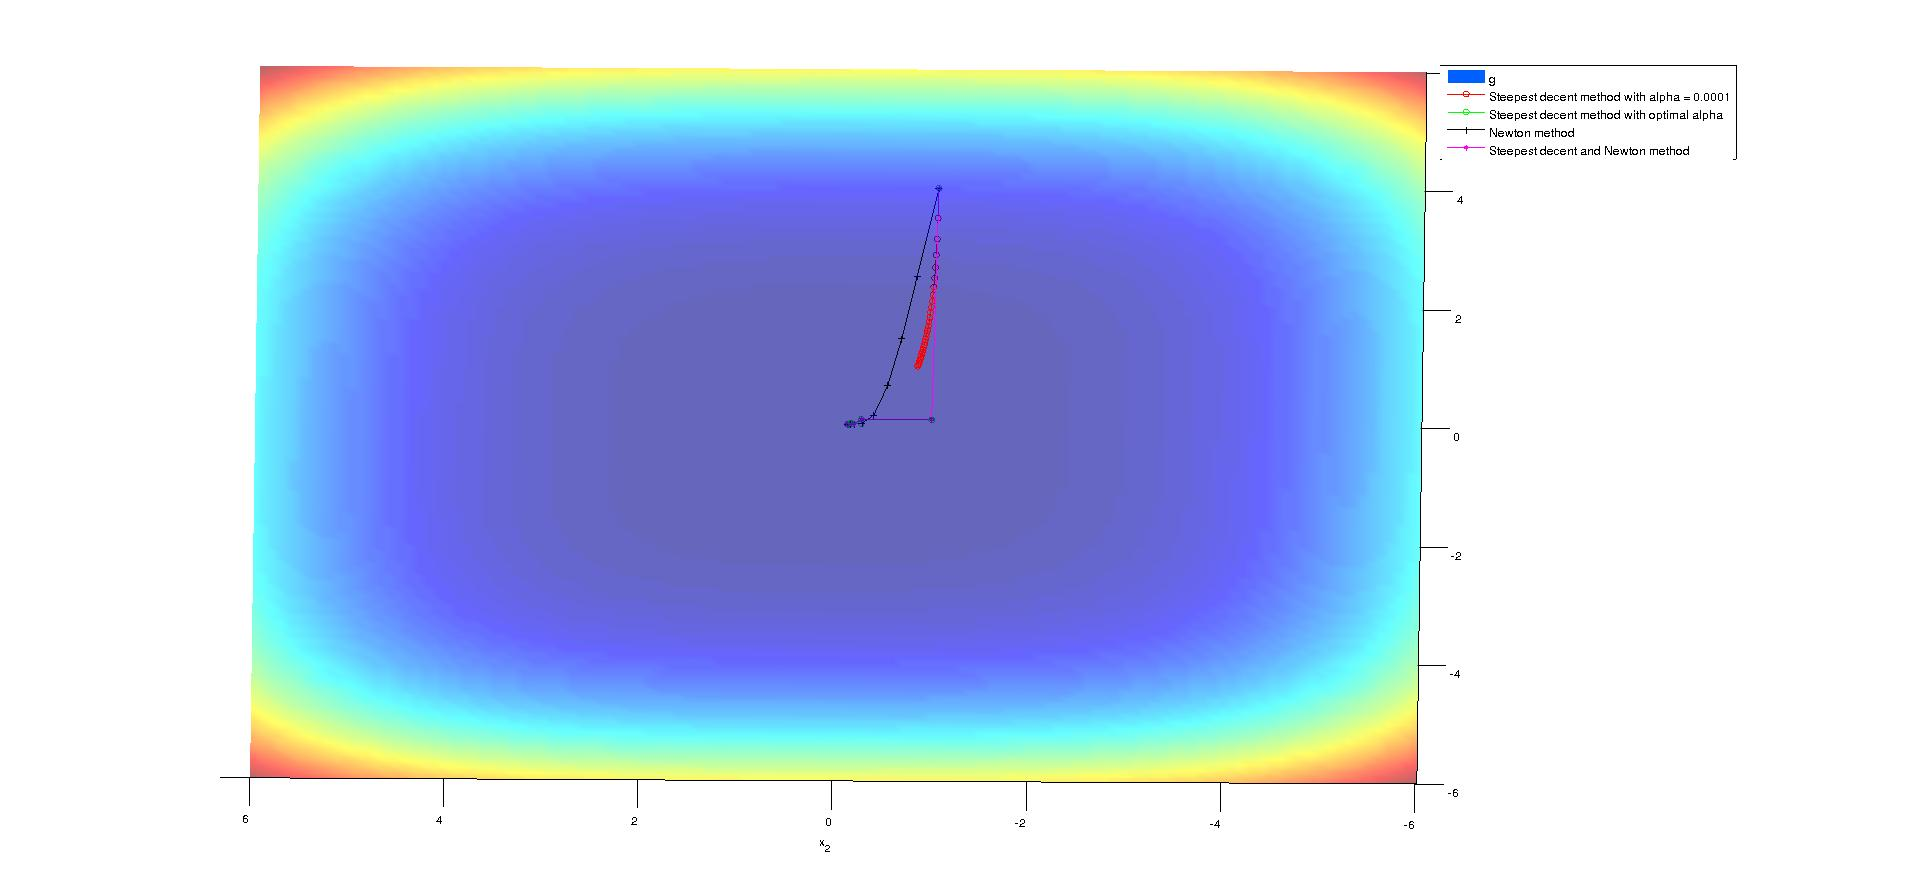
\includegraphics[width=\textwidth]{g.jpg}
	\caption{The function $g$.}
\end{figure}
\begin{figure}\label{gvalue}
	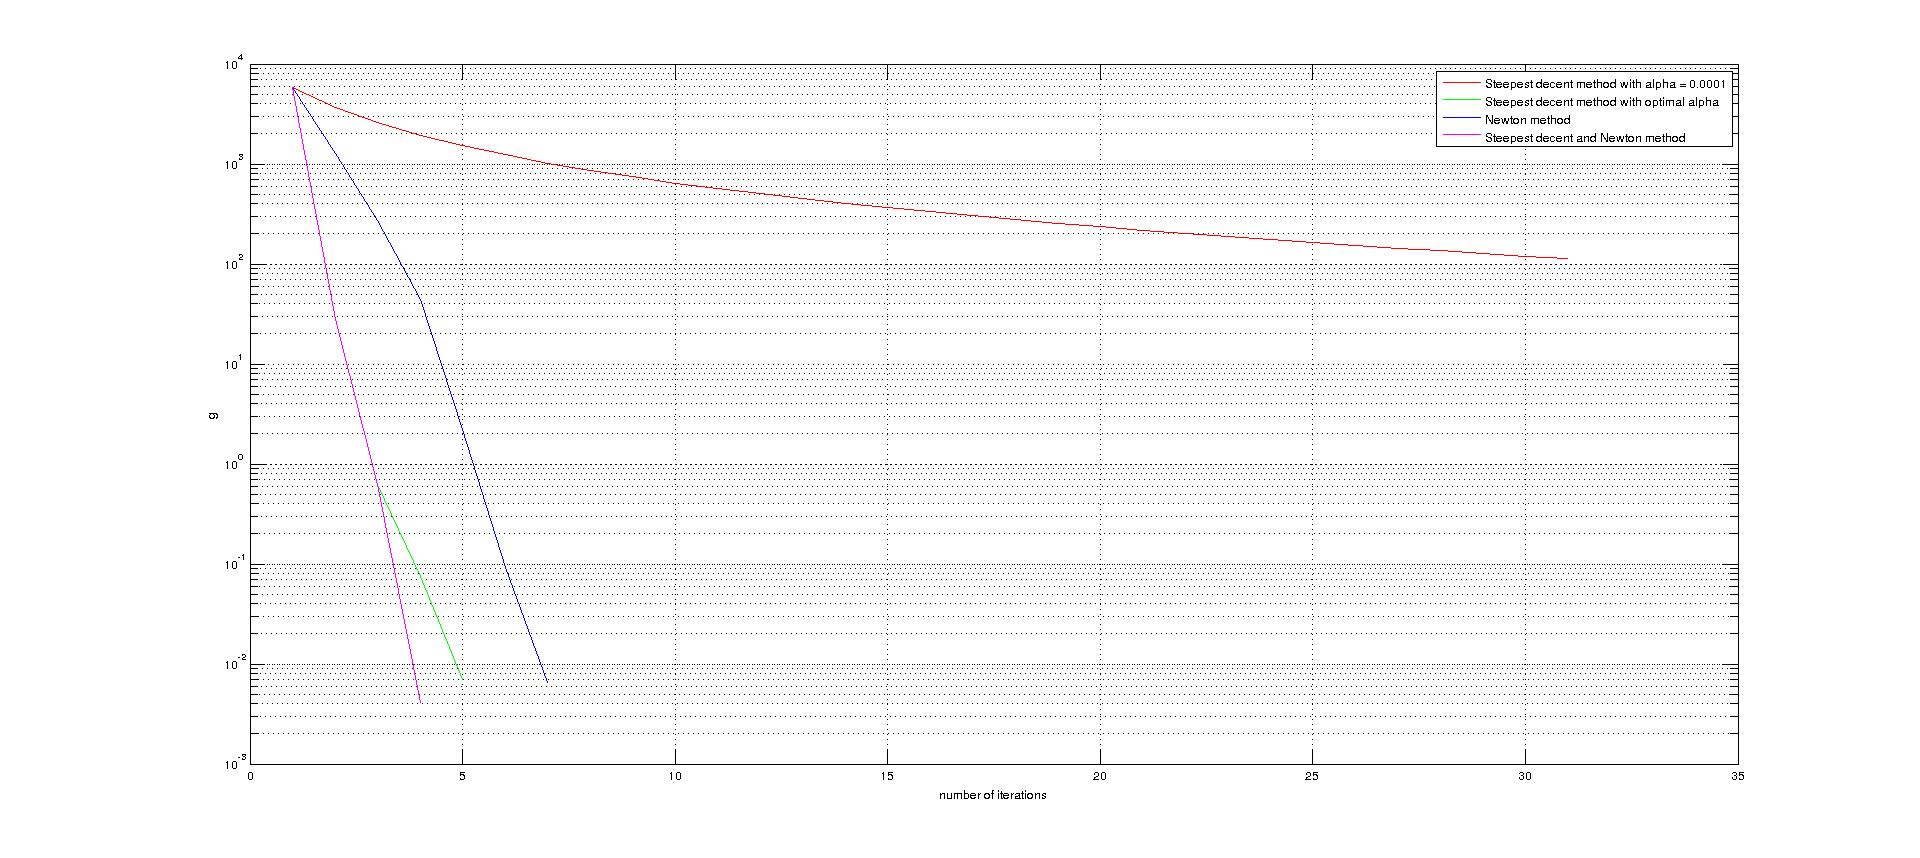
\includegraphics[width=\textwidth]{gvalues.jpg}
	\caption{The value of $g$ as a function of iterations for various methods.}
\end{figure}
\begin{figure}\label{res}
	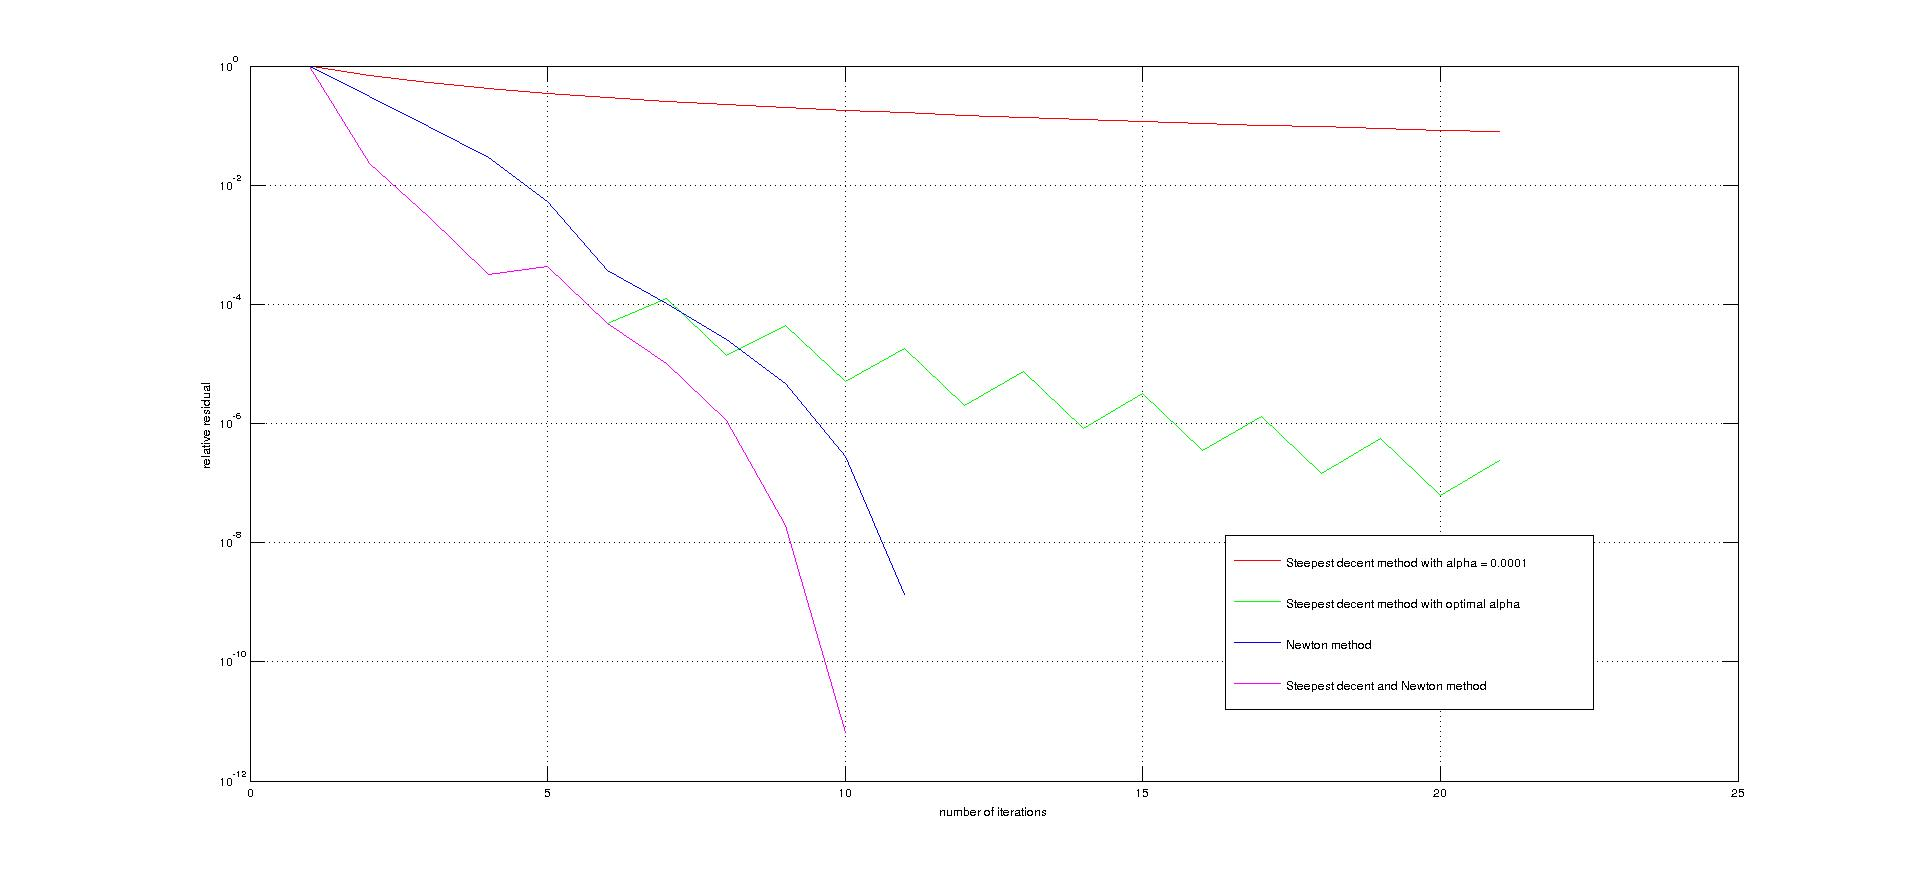
\includegraphics[width=\textwidth]{res.jpg}
	\caption{The relative residuals as a function of iterations for various methods.}
\end{figure}
\subsection{Steepest decent method with constant α}
The larger $|x|$, the smaller has to be α. % I cant understand this
If α is larger, the method does not converge any more.

The steepest decent method with constant α is alway interrupted when reaching the maximum number of iterations and not by reaching the tolerance for the residual.
For the starting value of $(4,-1)^T$, the algorithm needs $0.0957s$ for 1000 iterations, but is still not at the tolerance.


\subsection{Steepest decent method with optimal α}
The algorithm works better than with constant α, but when the relative residual drops below $10^{-3}$, the relative residual rises and falls alternately, but with a dropping drift.

\subsection{Newton method}
The relative residual obtained with the Newton method for relative residuals larger than $10^{-2}$ more iterations compared to the steepest decent method with optimal α.
On the other side the algorithm needs less iteration for small relative residuals.

\subsection{Steepest decent method and Newton method}
First the steepest decent method is applied and after a certain tolerance limit, the algorithm switches to the Newton method, to obtain the best result.

To find this tolerance limit, the total time for the algorithm is watched with various tolerance limits.
3 times each
\begin{tabular}{l|c|c|c|c|c|c|c|c}
tolerance limit & $10^{-1}$& $10^{-2}$& $10^{-3}$& $10^{-4}$& $10^{-5}$& $10^{-6}$\\\hline
time $[ms]$		& 1.37&1.06&1.26&1.54&2.17&2.97
\end{tabular}

The optimal tolerance limit is therefore...
We decided to keep the number of iterations constant, because 20 iterations is not much. 




\section{Your text, Im not sure if we should write that in our protocol}
All the values of the table are average values of a 1000 values sample, calculated from the starting point [4;-1].
As we can see, regardless of the tolerance and the maximun number of iterations, Newton's method is the fastest method. 
When we have a large number of iterations, the combination of steepest and Newton's method is the most precise (smallest residual). 
For this last method, the precision is increasing while the tolerance is decreasing but obviously, the cputime increases too.
The first method, steepest descent with arbitrary alpha appears to be the worst method. Indeed, the cputime and the residual are greater there. 
But, what is the interest of steepest method with the optimal alpha ? 
Actually, this method gives us a precise idea of where is the minimum of the function, without being very precise. 
The Newton's method can give us the same idea, but if we start far from the answer, the time of execution will be very higher. 
Moreover, if there are several points where the gradient equals to zero, we can't be sure that we are precisely in a global minimum or a local extremum. 
That is why it seems to be very useful to combine the two methods, because with the steepest descent we approach the solution to a certain point (and we are sure that is the solution) and with the Newton's method applied to this point we can go much more closer to the minimum. 
For instance, here with the tolerance 10e-6 and 1000 iterations, the precision of the Newton-steepest method is 1 million times more precise than the Newton's method alone. 


 As a conclusion, we have to choose the method accorded to the result we expect :
 if we just want a quick idea of the solution, we can just use the steepest descent with an alpha, arbitrary or optimal. But, if we prefer to be certain of the solution, we have to mix Newton's and steespest methods.
The Newton's method is between the last ones : 
very fast and quite precise but we cannot be completely sure of the solution, given that it will converge to the closest zero." 

\end{document}
